\documentclass[11pt,reqno]{amsart}

\usepackage{amsmath, amsfonts, amssymb,  mathrsfs,  array, stmaryrd,  indentfirst, amsthm,  hyperref, comment}
\usepackage{graphicx, enumitem, tabularx}

\usepackage[margin=1.0in]{geometry}
\usepackage{setspace}
\usepackage{mathtools}
\usepackage{float}
%\onehalfspacing

\setlength{\parskip}{8pt}

\numberwithin{equation}{section}
\theoremstyle{plain}
\newtheorem{lemma}{Lemma}[section]
\newtheorem{thm}{Theorem}[section]
\newtheorem{dfn}{Definition}[section]
\newtheorem{prop}{Proposition}[section]
\newtheorem{cor}{Corollary}[section]
\newtheorem{assumption}{Assumption}[section]
\newtheorem{rem}{Remark}[section]
\newcommand{\ab}[1]{\langle #1\rangle}
\newcommand{\snorm}[1]{\| #1\|_\infty}
\newcommand{\cadlag}{c\`{a}dl\`{a}g }
\newcommand{\lbar}[1]{\underline{#1}}
\newcommand{\ubar}[1]{\overline{#1}}
\newcommand{\Ito}{It\^{o}}
\newcommand\numberthis{\addtocounter{equation}{1}\tag{\theequation}}
\newcommand{\rom}[1]{\uppercase\expandafter{\romannumeral #1\relax}}
\renewcommand {\thefigure} {\thesection{}.\arabic{figure}}
\DeclareMathOperator*{\argmax}{arg\,max}
\DeclareMathOperator*{\argmin}{arg\,min}

\makeatletter
\def\@setcopyright{}
\def\serieslogo@{}
\makeatother

\begin{document}
\section{Theoretical Analysis}
While the analysis of Algorithm 4 seems within reach, there are some complications due to
the fact that points near the intersection may form a cluster of their own. See figure \ref{fig1}.
The vertical line and $\infty$-shaped line are sccessfully separated by Algorithm 4 ($K = 2$, $r = 15.0$, $\epsilon = 15.0$, $\eta = 0.3$).
But points near the intersectionis are fully classified as "Blue" group. 
\begin{figure}[htbp]
\centering
\vspace{-1em}
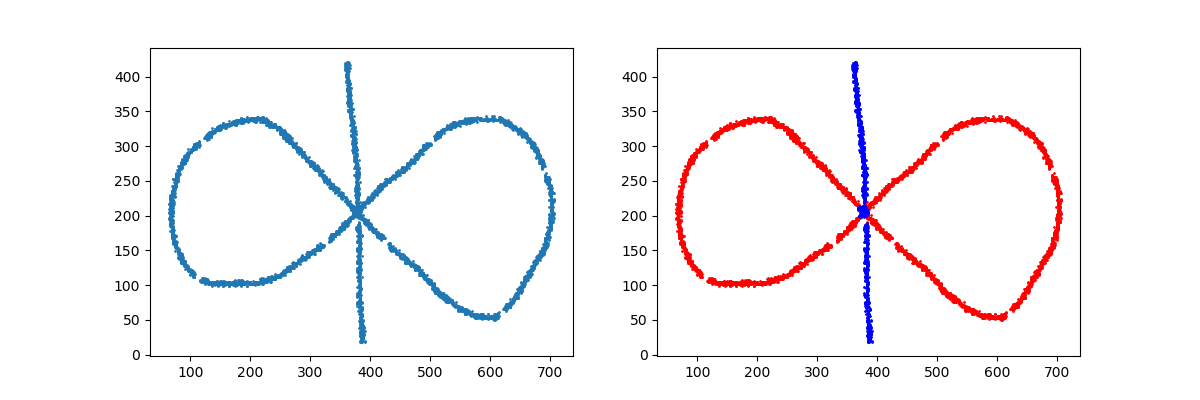
\includegraphics[width=1.0  \textwidth]{infinity_shape.png}
\vspace{-2em}
\caption{Example of intersection cluster}
\label{fig1}
\end{figure}

Instead, the authors mainly focus on some simpler variants described in Algorithm 2
and Algorithm 3, and then give a comment on the analysis of Algorithm 4. More theoretical results on intersecting manifolds 
refer to \cite{EAC},\cite{GCGL},\cite{MSEJC}. The generative model is a natural mathematical framework for multi-manifold learning where points are sampled in the vicinity of smooth surfaces embedded in Euclidean
space. One can see in the numerical experiments that the Algorithm 4 fails to deal with phenomenon that the intersection with a sharp corner. See figure \ref{fig2}. This is obtained by  Algorithm 4  ($K = 3$, $r = 10.0$, $\epsilon = 10.0$, $\eta = 0.5$), and is a typical result of this algorithm, where "2" is separated by the bottomleft sharp corner.
\begin{figure}[htbp]
\centering
\vspace{-1em}
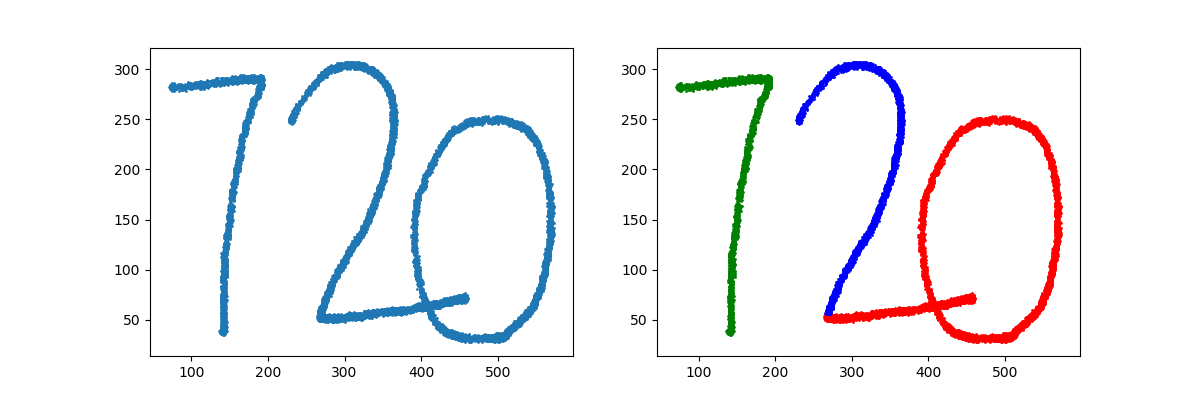
\includegraphics[width=1.0  \textwidth]{sharp_720.png}
\vspace{-2em}
\caption{Failure at the corner}
\label{fig2}
\end{figure}

To clarify the characteristics of the algorithm, additional "720"-shaped data which were written intentionally smoothly are applied below.  See figure \ref{fig3}, where both of the above and below are obtained by Algorithm 4 with the same parameters $K = 3$, $r = 10.0$, $\epsilon = 10.0$, $\eta = 0.5$. Due to smoothness, "720" are sccessfully separated into 3 digits in both figures.

\begin{figure}[htbp]
\centering
\vspace{-1em}
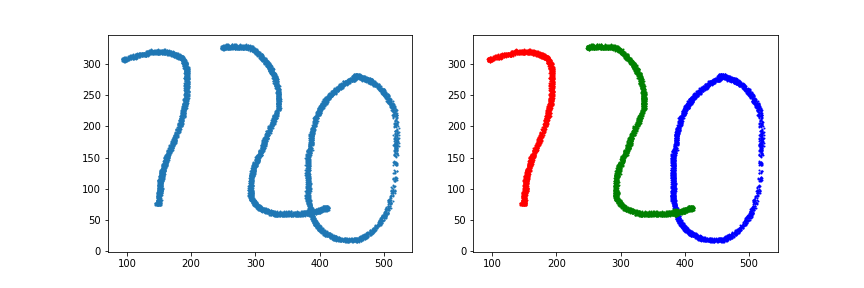
\includegraphics[width=1.0  \textwidth]{smooth_720_1.png}
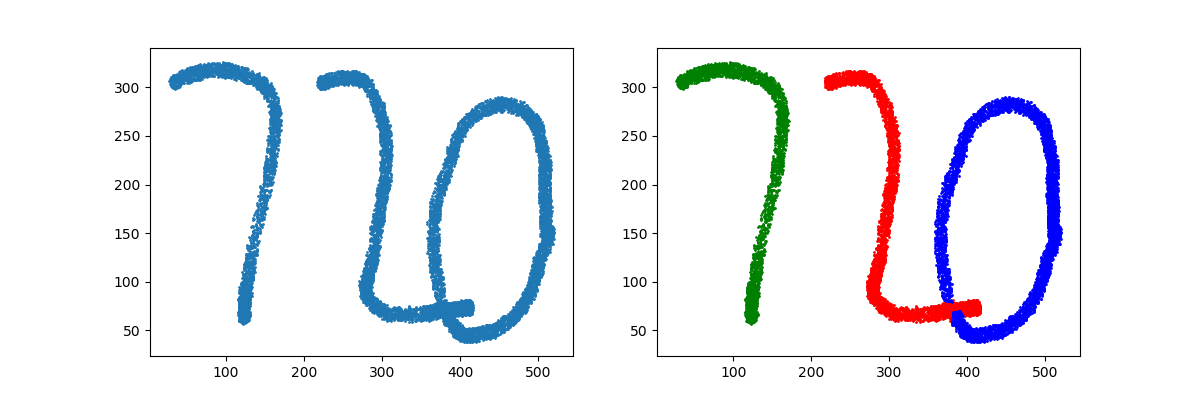
\includegraphics[width=1.0  \textwidth]{smooth_720_2.png}
\vspace{-2em}
\caption{Successful results with smooth data}
\label{fig3}
\end{figure}

Precisely, $K=2$ and each surface is a connected, $C^2$ and compact submanifold without boundary
and of dimension $d$ embedded in $\mathbb R^D$. Any such surface has a positive reach, which is what
we use to quantify smoothness. The clusters are generated as follows. Each data point $x_i$
is drawn according to
$$
x_i = s_i + z_i
$$
where $s_i$ is from the uniform distribution over $S_1\cup S_2$ and $z_i$ is an additive noise
term satisfying $||z_i||\le \tau$. The main theorem of the paper is given below.
\begin{thm}
Consider two connected, compact, twice continuously differentiable submanifolds
without boundary, of same dimension d, intersecting at a strictly positive angle, with
the intersection set having strictly positive reach. Assume the parameters are set so that
$$
\tau\le \frac{r\eta}{C},\ \ r\le\frac{\epsilon}{C},\ \ \epsilon\le\frac{\eta}{C},\ \ \eta\le\frac{1}{C}
$$
for large constant $C\ge 1$. Then with probability
at least $1-Cn\exp(- nr^d\eta^2/C)$:
\begin{itemize}
\item Algorithm 2 returns exactly two groups such that two points from different clusters are
not grouped together unless one of them is within distance Cr from the intersection.
\item Algorithm 3 returns at least two groups, and such that two points from different clusters
are not grouped together unless one of them is within distance Cr from the intersection.
\end{itemize}
\end{thm}
\begin{proof}
We give a sketch of proof of algorithm 2 and refers to the paper for more details. Some important notation:
$$
I^*=\{i: K_j=K_i,\ \forall j\in\Xi_i  \},\ \ \ \Xi_i=\{j\ne i, s_j\in N_r(s_i)   \}
$$
Thus $I^*$ indexes the points whose neighborhoods do not contain points from the other cluster.

\begin{enumerate}
\item Assume $\tau=0$, and then explain for how things change for $\tau>0$. Deriving a concentration inequality for local covariances with large constant $C$.
\item Then show that among points away from the intersection, those that are in the same cluster are neighbors in the graph if
they are within distance $\epsilon$, while those in different clusters cannot be neighbors in the graph.
\item Confirming that step 2 in algorithm 2 can eliminate all points which are not included in $I^*$, and  the points removed are within distance $Cr$ of the intersection, furthermore,  points removed are within distance $Cr$ of the intersection.
\item Concluding that in step 4, algorithm 2 returns two graphs, and each group covers an entire cluster except for points within distance $O(r)$ of the intersection.
\end{enumerate}
\end{proof}
To conclude, the key point of the approach is using principal component analysis to study the local behavior of data, and then use the information about affinity to generate a new local  neighborhood graph. However, the selection of the parameters is quite sensitive to the final output, it is still a quite acceptable approach in many applications and perform well in particular example.

For comparison, results with different parameters are described in figure \ref{fig4}, \ref{fig5}, and \ref{fig6}. If not explicitly mentioned, parameters $K = 3$, $r = 10.0$, $\epsilon = 10.0$, $\eta = 0.5$ are used.

\begin{figure}[htbp]
\centering
\hspace{-2em}
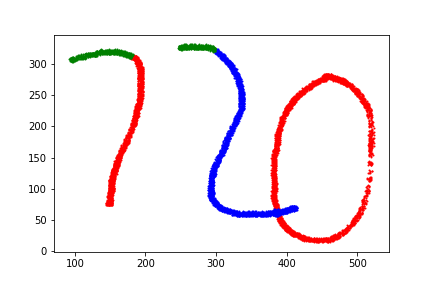
\includegraphics[width=0.37  \textwidth]{eta_small.png}
\hspace{-2em}
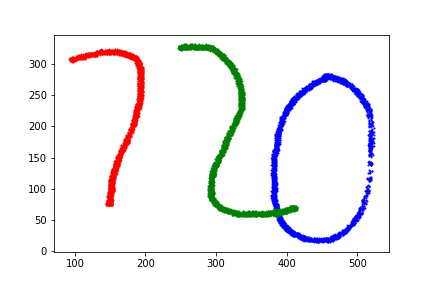
\includegraphics[width=0.37  \textwidth]{normal_720.png}
\hspace{-2em}
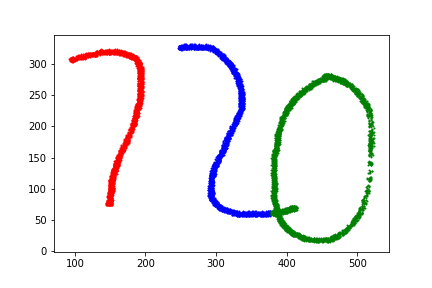
\includegraphics[width=0.37  \textwidth]{eta_large.png}
\hspace{-2em}
\vspace{-1em}
\caption{[Left]: $\eta = 0.1$,  [Middle]: $\eta = 0.5$,  [Right]: $\eta = 1.0$}
\label{fig4}
\end{figure}
\begin{figure}[htbp]
\centering
\vspace{-1em}
\hspace{-2em}
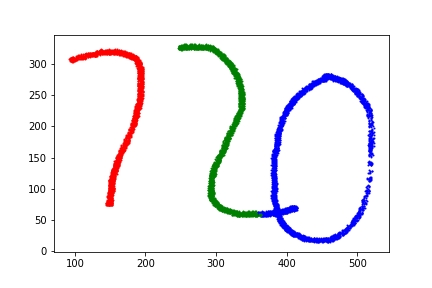
\includegraphics[width=0.37  \textwidth]{r_small.png}
\hspace{-2em}
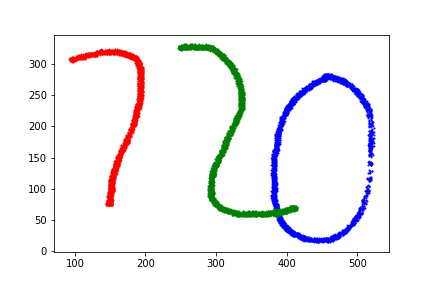
\includegraphics[width=0.37  \textwidth]{normal_720.png}
\hspace{-2em}
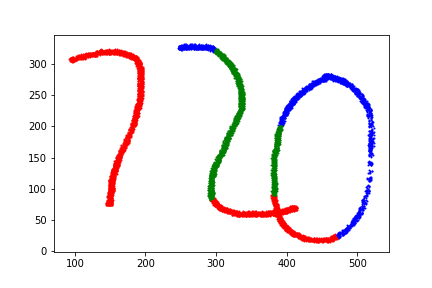
\includegraphics[width=0.37  \textwidth]{r_large.png}
\hspace{-2em}
\vspace{-1em}
\caption{[Left]: $r = 3.0$,  [Middle]: $r = 10.0$,  [Right]: $r = 40.0$}
\label{fig5}
\end{figure}
\begin{figure}[htbp]
\centering
\vspace{-1em}
\hspace{-2em}
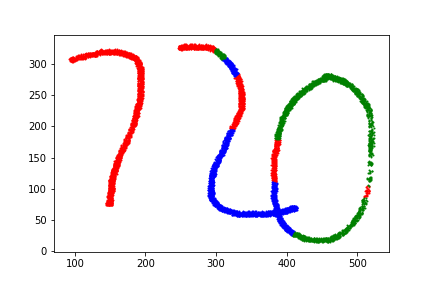
\includegraphics[width=0.37  \textwidth]{eps_small.png}
\hspace{-2em}
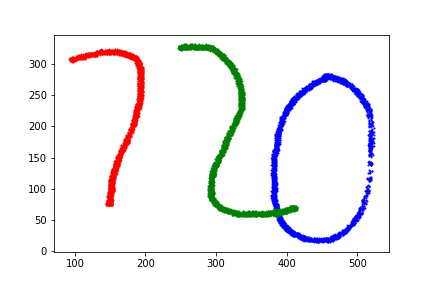
\includegraphics[width=0.37  \textwidth]{normal_720.png}
\hspace{-2em}
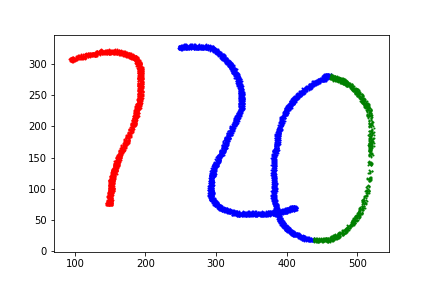
\includegraphics[width=0.37  \textwidth]{eps_large.png}
\hspace{-2em}
\vspace{-1em}
\caption{[Left]: $\epsilon = 3.0$,  [Middle]: $\epsilon = 10.0$,  [Right]: $\epsilon = 40.0$}
\label{fig6}
\end{figure}


When $\eta$ is small, local directions of data tend to have a more important role in clustering than geometric closeness between data.
In fact, in figure \ref{fig4} [Left], only horizontal parts of "7" and "2" are labeled as green. On the other hand, in figure \ref{fig4} [Right], the orthogonal intersection doesn't work as a separating point between the vertical and the horizontal, and then a part of "2" is absorbed in "0".

$r$ should be chosen so that small circles with radious $r$ can appropriately cover the thickness of lines or surfaces of data points. If $r$ is too small, the small circles may be buried in lines or surfaces. If $r$ is too large, some circle may totally wrap around a intersection. In both cases, the classification will fail as described in figure \ref{fig5} [Left] and [Right]. Figure \ref{fig7} shows an enlarged view of the boundary between the blue and green areas in figure \ref{fig5} [Left]. A small green circle buried in the line can be seen here.

\begin{figure}[htbp]
\centering

\includegraphics[width=0.3  \textwidth]{boundary.png}
\vspace{-1em}
\caption{Small green circle buried in the line}
\label{fig7}
\end{figure}

When $\epsilon$ is small, the affinity based on geometric distance decays immediately. Therefore it is natural that figure \ref{fig6} [Left] has a mottled  pattern. Conversely, when $\epsilon$ is large, the affinity remains higher over a wide distance.

\begin{thebibliography}{}
\bibitem{EAC} 
E. Arias-Castro. Clustering based on pairwise distances when the data is of mixed dimensions.
IEEE Transactions on Information Theory, 57(3):1692 –1706, 2011.
\bibitem{GCGL}
G. Chen and G. Lerman. Foundations of a multi-way spectral clustering framework for
hybrid linear modeling. Foundations of Computational Mathematics, 9(5):517–558, 2009b.
\bibitem{MSEJC}
M. Soltanolkotabi and E. J. Cand\'es. A geometric analysis of subspace clustering with
outliers. Annals of Statistics, 40(4):2195–2238, 2012.
\end{thebibliography}

\end{document}